\chapter{Vector Calculus: What is the fastest way downhill?} \label{apx:vcalc}

\section{The $\grad$ (del) operator}

The differential operator, del ($\nabla$), is a convenient way to represent
multiple partial derivatives in a compact form.  Several operations are common
using $\nabla$: the gradient ($\mbox{grad}$) of a scalar function, $f$, is given
by
\begin{equation}
    \mbox{grad}\; f(x,y,z) = \grad f = \pdv{f}{x}\vu{x} + \pdv{f}{y}\vu{y} +
        \pdv{f}{z}\vu{z},
\end{equation}
which yields a vector with direction of the indicated by the unit vectors
$(\vu{x}, \vu{y}, \vu{z})$; the divergence ($\mbox{div}$) of a vector
function, $\vb{A}$, is given by
\begin{equation}
    \mbox{div}\; \vb{A}(x,y,z) = \div \vb{A} =
        \pdv{A_x}{x} + \pdv{A_y}{y} + \pdv{A_z}{z},
\end{equation}
which yields a scalar; and the curl of a vector function is given by
\begin{equation}
    \mbox{curl}\; \vb{A}(x,y,z) = \curl \vb{A} = 
        \left( \pdv{A_z}{y} - \pdv{A_y}{z} \right) \vu{x} +
        \left( \pdv{A_x}{z} - \pdv{A_z}{x} \right) \vu{y} +
        \left( \pdv{A_y}{x} - \pdv{A_x}{y} \right) \vu{z},
\end{equation}
which yields a vector.  Because the definition of the curl can be difficult to
remember, it can also be represented as the determinant,
\begin{equation*}
    \curl \vb{A} =
    \begin{vmatrix}
        \vu{x} & \vu{y} & \vu{z} \\
        \pdv{}{x} & \pdv{}{y} & \pdv{}{z} \\
        A_{x} & A_{y} & A_{z}
    \end{vmatrix}
    = \left( \pdv{A_z}{y} - \pdv{A_y}{z} \right) \vu{x} +
    \left( \pdv{A_x}{z} - \pdv{A_z}{x} \right) \vu{y} +
    \left( \pdv{A_y}{x} - \pdv{A_x}{y} \right) \vu{z},
\end{equation*}

A graphical description of the divergence and curl of a
vector field in relation to a point are illustrated in Figure~\ref{fig:divcurl}.
\begin{figure}[hbt]
  \centering
  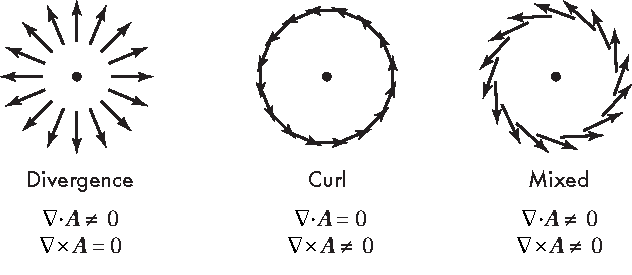
\includegraphics[]{math_primer/figures/div_grad_curl.pdf}

  \caption{The divergence and curl of a vector field.  The terms convergence
  (now divergence) and curl were actually suggested by Maxwell for vector
  operations.  The vector field on the left exhibits pure divergence; all the
  vectors point normal to the point.  The vector field in the center illustrates
  pure curl; all the vectors are parallel the point inducing a circulation about
  the point.  The vector field on the right is mixed with both non-zero
  divergence and curl.}
  \label{fig:divcurl}
\end{figure}

Another important relation is the Laplacian operator and is particularly useful
in potential fields,
\begin{equation}
    \div \grad f = \nabla^{2} f = \pdv[2]{f}{x} + \pdv[2]{f}{y} + \pdv[2]{f}{z}.
\end{equation}
For a thorough (but quite readable) treatment of the $\nabla$ operator, I refer
you to \citet{Schey1997}.

These terms (other than Laplacian) were devised because they attempt to convey a
physical meaning to the mathematics.  Consider the topography of a mountain.
Every point on the mountain can be thought of in terms of the elevation of that
point.  The collection of the elevation points is a scalar function or scalar
`field' that we of course call the topography.  The gradient of the topography
is simply the slope at a given point.

Taking our topography example, lets place a marble at every point on the
surface.  The marbles are instantaneously moving down the direction of the
maximum slope.  At a local high point, a peak, all the marbles nearest the peak
are moving away from each other or diverging.  At a local low, a valley, all the
marbles are moving towards each other (converging).  The divergence tells us how
much the velocity fields concentrate or disseminate the marbles.

It is a bit more difficult to come up with an example of the curl using our
topography example.  Instead think of a pinwheel in the wind.  As the wind
blows, the point on the pinwheel tries to move in the direction of the wind is
blowing but cannot because it is attached to the surface.  The force of the wind
against this point then imparts a torque about the point causing a net rotation
(or curl).

There are some vector identities that can be derived from various combinations of
the $\nabla$ operator.  One that we use in EM geophysics is
\begin{equation}
    \curl \curl \vb{A} = \grad(\div \vb{A}) - \nabla^{2} \vb{A}.
    \label{eq-curlcurl}
\end{equation}

\section{Contour Integrals} \label{apx:cintegral}
The integral form of Maxwell's equations uses notation $\fint{C}{}$\ or
$\fint{S}{}$, in several places which denote a line integral and surface
integral, respectively.  When the line (contour) or surface are enclosed
$\cint{}$\ is used, and is only valid when the entire path or surface are
included in the integration.

\bibliographystyle{elsarticle-harv}
\bibliography{ref}
